\documentclass[../classical_mechanics.tex]{subfiles}

\begin{document}

    \section{The Conservation of Energy}\label{sec:conservation-of-energy}
        % TODO: introduce kinetic energy as integral of momemtum?
        Lets calculate the rate of change of velocity squared.
        \begin{align}
            \dv{}{t}v^2&=\dv{\vec{v}}{t}\cdot\vec{v}+\vec{v}\cdot\dv{\vec{v}}{t}\\
            &=2\vec{v}\cdot\dv{\vec{v}}{t}\\
            &=2\vec{v}\cdot\frac{\vec{F}}{m},
        \end{align}
        where in the last line we have used Newton II. Thus,
        \begin{equation}
            \dv{}{t}\left(\frac{1}{2}mv^2\right)=\vec{F}\cdot\vec{v}.
        \end{equation}
        We define the quantity in parentheses as the kinetic energy.
        \begin{definition}
            \textbf{Kinetic energy} is given by
            \begin{equation}
                K=\frac{1}{2}mv^2.
            \end{equation}
        \end{definition}
        Let's see how the kinetic energy changes for a given force. We can find the change in kinetic energy by integrating:
        \begin{align}
            \int_{t_1}^{t_2}\dv{}{t}\left(\frac{1}{2}mv^2\right)\dd{t}&=\frac{1}{2}m(v(t_2)^2-v(t_1)^2)\\
            &=\Delta K=\int_{t_1}^{t_2}\vec{F}\cdot\vec{v}\dd{t}.
        \end{align}

        Consider the gravitational force $\vec{F}=-mg\khat$. Then
        \begin{align}
            \int_{t_1}^{t_2}\dv{}{t}\left(\frac{1}{2}mv^2\right)\dd{t}&=\frac{1}{2}m(v(t_2)^2-v(t_1)^2)\\
            &=\int_{t_1}^{t_2}\vec{F}\cdot\vec{v}\dd{t}\\
            &=-\int_{t_1}^{t_2}mgv_z\dd{t}\\
            &=-mg(z(t_2)-z(t_1)),
        \end{align}
        and hence,
        \begin{equation}
            \frac{1}{2}mv_1^2+mgz_1=\frac{1}{2}mv_2^2+mgz_2.
        \end{equation}
        So this quantity is \textbf{constant} over the path of the object (since $t_1$ and $t_2$ were arbitrary).
        If we write
        \begin{equation}
            K=\frac{1}{2}mv^2,\quad U_g=mgz,
        \end{equation}
        then we have
        \begin{equation}
            E=K+U_g.
        \end{equation}
        \begin{example}
            Consider a pendulum on the end of a string. What is the maximum speed that the pendulum attains as it swings?
            % TODO: write this
        \end{example}
        \begin{example}[The Epitaph of Stevinus]
            Consider a chain of uniform density draped over a trianglular block.
            % TODO: add diagram for this
            If the chain is free to move with no friction, will it fall to the left, right, or will it balance in place.

            The answer is that the chain will not move.
            We will prove this three different ways.
            The first way by analysing the forces as we have learned in chapter~\ref{chap:laws-of-motion}, the second way using energy conservation, and the third way using a clever 16\ts{th} century thought experiment.

            To prove that there is no movement using forces, we will look at the components of the weight parallel to the incline for the left and right halves of the chain separately and show that they are equal in magnitude --- therefore the total force must be zero.
            First, note that if the total mass of the chain is $m$, then the magnitude of the weight force on the left side is $\frac{3}{7}mg$ and on the right it is $\frac{4}{7}mg$.
            % TODO: add free body diagrams
            On the left, the $x$-component of weight is $\frac{3}{7}mg\cos\theta$ and on the right it is $\frac{4}{7}mg\sin\theta$.
            Using trigonometry, we have that
            \begin{equation}
                \cos\theta=\frac{4}{5},\quad\sin\theta=\frac{3}{5},
            \end{equation}
            and therefore
            \begin{equation}
                F_\text{left}-F_\text{right}=\frac{3}{7}mg(\frac{4}{5})-\frac{4}{7}mg(\frac{3}{5})=0.
            \end{equation}

            To use energy conservation, we will first restate the problem slightly.
            Instead of a chain draped over the whole wedge, suppose that left and right sides of the chain are replaced with blocks of equivalent mass located at the centre of masses of each part.
            The blocks are connected with a light inextensible string which runs over the top of the wedge via a frictionless pulley.
            % TODO: include diagram for this
            Now, we can calculate the total energy before the system starts moving, given by the sum of gravitational potential energy of each part (we set the zero point to be the bottom of the wedge):
            \begin{align}
                E_\text{before}=U_L+U_R&=\frac{3}{7}mgh_L+\frac{4}{7}mgh_R\\
                &=\frac{3}{7}mg(\frac{3}{2}\cos\theta)+\frac{4}{7}mg(2\sin\theta)\\
                &=\frac{18}{35}mg+\frac{24}{35}mg=\frac{6}{5}mg.
            \end{align}
            Suppose the system moves.
            Then at a later instant the blocks will have a collective velocity $v$, the left block will have moved a distance $l$ along the incline, and the right block will have moved $-l$.
            The total energy at this time is
            \begin{align}
                E_\text{after}=U_L^\prime+U_R^\prime+K&=\frac{3}{7}mgh_L^\prime+\frac{4}{7}mgh_R^\prime+\frac{1}{2}mv^2\\
                &=\frac{3}{7}mg\left(\frac{3}{2}+l\right)\cos\theta+\frac{4}{7}mg(2-l)\sin\theta+\frac{1}{2}mv^2\\
                &=\frac{18}{35}mg+\frac{12}{35}mgl+\frac{24}{35}mg-\frac{12}{35}mgl+\frac{1}{2}mv^2\\
                &=\frac{6}{5}mg+\frac{1}{2}mv^2.
            \end{align}
            Since energy is conserved, we should have $E_\text{before}=E_\text{after}$, which implies that
            \begin{equation}
                \frac{1}{2}mv^2=0,\quad\implies v=0.
            \end{equation}

            Finally, we will prove this using a thought experiment by Flemish scientist Simon Stevin.
            % TODO: include a diagram of this
            Suppose we attach another length of chain to both ends such that it forms a closed loop, with the new section hanging freely below the wedge.
            Since it hangs symmetrically, the forces on both sides (the tension at the lower vertices of the wedge) must be equal.
            If the forces on the upper part of the wedge were unbalanced, the whole loop would begin to rotate around the wedge in perpetual motion.
            This cannot happen, thus the forces on the upper part must be balanced.
            This proof is known as the Epitaph of Stevinus.
        \end{example}

    \section{Work}\label{sec:work}
        As force is applied to an object, energy will be added or taken away.
        We call this energy \textbf{work}.
        Work is defined by the force applied multiplied by the distance the force was applied over.
        For a constant force, this can be written mathematically as $W=\vec{F}\cdot\vec{s}=\abs{\vec{F}}\abs{\vec{s}}\cos\theta$ (check that this has units of energy!).
        We can think of work as the mechanism for transferring energy.
        
        If the force is changing continuously over time, we need to be more careful about how we define the work.
        We break up the path of the object into small sections over which the force is approximately constant and integrate over all these small sections to get the total work.
        \begin{definition}
            The work done by a force over an infinitesimal distance $\dd{\vec{r}}$ is
            \begin{equation}
                \dd{W}=\vec{F}\cdot\dd{\vec{r}}.
            \end{equation}
            The total work is then defined as
            \begin{equation}\label{eq:work-line-integral}
                W=\int\dd{W}=\int_{\vec{r}_1}^{\vec{r}_2}\vec{F}\cdot\dd{\vec{r}},
            \end{equation}
            where $\vec{r}_1$ and $\vec{r}_2$ are the start and end points of the path being integrated over.
        \end{definition}
        This is a line integral, so evaluating it will involve choosing a coordinate system and splitting the path up into components along each axis.
        Let's do a couple of examples now.
        
        In cartesian coordinates, the force vector is given by $\vec{F}=F_x\ihat+F_y\jhat+F_z\khat$ and the infinitesimal displacement is $\dd{\vec{r}}=\dd{x}\ihat+\dd{y}\jhat+\dd{z}\khat$.
        The dot product $\vec{F}\cdot\dd{\vec{r}}$ is $F_x\dd{x}+F_y\dd{y}+F_z\dd{z}$.
        Thus, the integral in equation~\ref{eq:work-line-integral} becomes
        \begin{equation}
            W=\int_{x_1}^{x_2}F_x\dd{x}+\int_{y_1}^{y_2}F_y\dd{y}+\int_{z_1}^{z_2}F_z\dd{z},
        \end{equation}
        where the limits of the integrals are the components of the start and end points of the path.
        \begin{example}\label{ex:work-cartesian}
            Consider a force $\vec{F}=xy\ihat+x^2y\jhat$.
            What is the work done on an object that moves along a straight line from $(0,0)$ to $(4,3)$ while under the influence of this force.
            % TODO: add diagram

            Note that the components of this force $F_x$ and $F_y$ both depend on $x$ and $y$, so to evaluate the integrals we will have to eliminate the other variable by parameterising the path.
            Luckily this is easy for a straight line, the path can be written as $y=\frac{3}{4}x$.
            Then the work is
            \begin{align}
                W&=\int_0^4 xy\dd{x}+\int_0^3x^2y\dd{y}\\
                &=\int_0^4 x\left(\frac{3}{4}x\right)\dd{x}+\int_0^3\left(\frac{4}{3}y\right)^2y\dd{y}\\
                &=\frac{3}{4}\int_0^4x^2\dd{x}+\frac{16}{9}y^3\dd{y}\\
                &=\left.\frac{1}{4}x^3\right|_0^4+\left.\frac{4}{9}y^4\right|_0^3\\
                &=\qty{52}{\joule}.
            \end{align}
        \end{example}
        
        Because work is defined by a line integral, its value may change depending on the path taken, even if the start and end points are the same.
        This is quite often the case.
        Let's do the above example again, but have the object follow a different path.
        \begin{example}
            Calculate the work done on an object under the influence of the force from example~\ref{ex:work-cartesian}, but this time following a path from $(0,0)$ to $(4,0)$, then to $(4,3)$.
            % TODO: add diagram

            We can break this path up into two separate straight lines to integrate over.
            The total work done is the sum of the work over both paths.
            Over the first part, $y=0$, so $F_x=xy=0$, so no work is done over this section of the path.
            For the second part, $x=4$ and the work done is
            \begin{equation}
                W=\int_0^3 16y\dd{y}=\left.8y^2\right|_0^3=\qty{72}{\joule}.
            \end{equation}
        \end{example}
        % That the work done is different should not be surprising.
        % Imagine you are trying to walk around in a gale.

        Now let's look at how to calculate work done in polar coordinates, in 2D to begin with.
        Force in polar coordinates is given by $\vec{F}=F_r\uvec{r}+F_\theta\uvec{\theta}$, and the infinitesimal displacement is $\dd{\vec{r}}=\dd{r}\uvec{r}+r\dd{\theta}\uvec{\theta}$.
        % TODO: add a derivation of infinitesimal displacement vector in polar coordinates (and a diagram)
        Thus the work done is given by
        \begin{align}
            W&=\int(F_r\uvec{r}+F_\theta\uvec{\theta})\cdot(\dd{r}\uvec{r}+r\dd{\theta}\uvec{\theta})\\
            &=\int_{r_1}^{r_2}F_r\dd{r}+\int_{\theta_1}^{\theta_2}F_\theta r\dd{\theta}\label{eq:work-integral-2d-polar}.
        \end{align}
        % TODO: add example 6.1 from notes here
        \begin{example}\label{ex:work-polar}
            
        \end{example}

    \section{Work-Energy Theorem}\label{sec:work-energy-theorem}
        As a force does work on an object, its speed will increase or decrease.
        This relationship is clarified by the work-energy theorem.
        % TODO: write more detailed intro to the work-energy theorem here
        \begin{theorem}[Work-Energy Theorem]
            The net work on an object is equal to the change in its kinetic energy.
            \begin{align}
                W&=\int_\mathrm{path}\mathrm{d}W\\
                &=\int_{r_1}^{r_2}\vec{F}\cdot\mathrm{d}\vec{r}\\
                &=\int_{t_1}^{t_2}\vec{F}\cdot\frac{\mathrm{d}\vec{r}}{\mathrm{d}t}\mathrm{d}t\\
                % TODO: could also write F as d(mv)/dt (NII)
                &=\int_{t_1}^{t_2}\vec{F}\cdot\vec{v}\mathrm{d}t\\
                &=\int_{t_1}^{t_2}\frac{\mathrm{d}}{\mathrm{d}t}\left(\frac{1}{2}mv^2\right)\mathrm{d}t=\Delta K.
            \end{align}
        \end{theorem}
        The kinetic energy depends on the speed of the object, so if the net work is $>0$ then the object must have sped up.
        Likewise, if the net work is $<0$, the object has slowed down.
        If the net work is 0, the object must be at the same speed that it started at.
        \begin{example}
            Consider a particle of mass $\qty{2}{\kilogram}$.
            It is being acted on by a force with the form $\vec{F}=4x\ihat$, and at $t=0$ its position is $x=\qty{4}{\meter}$ and its velocity is $v_0=\qty{1}{\meter\per\second}$.
            What is the particle's velocity when it reaches $x=\qty{6}{\meter}$?

            We can solve this using the work energy theorem.
            First we calculate the work done:
            \begin{equation}
                W=\int_{x_1}^{x_2}F_x\dd{x}=\int_{4}^{6}4x\dd{x}=\left.2x^2\right|_4^6=\qty{40}{\joule}.
            \end{equation}
            Now we can use the fact that the work done is equal to the change in kinetic energy to get a formula for the final velocity:
            \begin{align}
                W&=\Delta K=\frac{1}{2}m(v_f^2-v_0^2)\\
                \implies v_f&=\sqrt{\frac{2W}{m}+v_0^2}\\
                &=\qty{6.4}{\meter\per\second}.
            \end{align}
        \end{example}
        % \begin{example}
        %     Consider a chain of length $L$ and total mass $m$ hanging over the edge of a frictionless table.
        %     % TODO: write this example from notes
        % \end{example}

        Now let's look at a mass on a spring. The restoring force on the mass always acts opposite to displacement. Hooke's law says
        \begin{equation}
            F_s=-k(x-x_0),
        \end{equation}
        % TODO: add diagram of system, free-body diagram and force vs displacement
        where $k$ is the spring constant, $x_0$ is the equilibrium position of the spring.
        Then the work done by the spring force is
        \begin{align}
            W_s=\int_{x_0}^{x_f}F_s(x)\dd{x}&=-\int_{x_0}^{x_f}k(x-x_0)\dd{x}\\
            &=-\frac{1}{2}k(x_f-x_0)^2.
        \end{align}
        Note that the work done is always negative no matter if the displacement is positive or negative because the force points in the opposite direction.
        Now we define the spring potential energy as
        \begin{equation}
            U_s=-W_s=\frac{1}{2}k(x_f-x_0)^2,
        \end{equation}
        Then by the work-energy theorem we have
        \begin{equation}
            \Delta K=W_s=-\Delta U_s,
        \end{equation}
        so
        \begin{equation}
            K+U_s=E
        \end{equation}
        is constant.
        % TODO: mention the sign of work. Given by F.dr, but also note that positive work ON an object INCREASES its kinetic energy
        % TODO: mention the relation between NIII and sign of work

        % TODO: include discussion of friction
        % TODO: show that total energy is not conserved when friction is considered
        % TODO: solve stopping distance of a block sliding down a slope example from chapter 1 using only energy conservation (or lack thereof in this case)

    \section{Conservative Forces}\label{sec:conservative-forces}
        We have seen that in some cases the total energy is conserved and in others it is not.
        As we have seen above, work done is defined by a line integral, so in general it depends on the path chosen for integration, which corresponds to the path of the object through space.
        However, we have seen for the case of gravity and the spring force that the work done depends \textit{only} on the initial and final positions; the integral is \textit{path independent}.
        We also saw that in this case we can define a potential energy function for which
        \begin{equation}
            W=\int_{r_1}^{r_2}\vec{F}\cdot\dd{\vec{r}}=-(U(r_2)-U(r_1)),
        \end{equation}
        where $\vec{F}=-\nabla U$ (mathematicians will note that this is just a special case of the \textbf{gradient theorem}, a multidimensional generalisation of the fundamental theorem of calculus).
        We call forces which have this property \textbf{conservative forces}.
        They are called this because by the work-energy theorem:
        \begin{equation}
            W=-(U(r_2)-U(r_1))=-\Delta U=\Delta K,
        \end{equation}
        and hence the total energy $E=K+U$ is conserved.

        To fully define a potential energy function, we must explicitly say where potential energy is zero.
        Suppose we choose the point $\vec{r}_0$, so $U(\vec{r}_0)=0$.
        Then we can define
        \begin{equation}
            U(\vec{r})=-\int_{\vec{r}_0}^{\vec{r}}\vec{F}\cdot\dd{\vec{r}}.
        \end{equation}
        We can choose whatever point is most convenient because it won't affect the physics, since force is minus the derivative of the potential energy any constant value we add to it will disappear.
        Only \textit{differences} in potential (potential difference) have physical significance.

        The gradient formula $\vec{F}=-\nabla U$ is the most general way to define potential energy, but it can be written more explicitly by choosing a coordinate system.
        For example, in 1D it reduces to
        \begin{equation}
            F=-\dv{U}{x},
        \end{equation}
        in 3D cartesian coordinates it is
        \begin{equation}
            \vec{F}=-\pdv{U}{x}\ihat-\pdv{U}{y}\jhat-\pdv{U}{z}\khat,
        \end{equation}
        in 2D polar coordinates it is
        \begin{equation}
            \vec{F}=-\pdv{U}{r}\uvec{r}-\frac{1}{r}\pdv{U}{\theta}\uvec{\theta},
        \end{equation}
        and so on.
        % TODO: add exersise for some coordinate system

        These discoveries unlock a very powerful and intuitive way to look at dynamics.
        Rather than looking at the force and trying to figure out at what points it is pushing in which direction, we can simply look at the graph of the potential energy, specifically the slope.
        For example, suppose a force has the following potential energy function as a function of radial distance $r$.
        % TODO: add diagram for this
        At the points B and D, the gradient is flat, so $\dv{U}{r}=0$ and $F=0$, there is no force at these points.
        At A and E we have a positive gradient, which means force is negative, and at C the gradient is negative which implies a positive force.
        We can immediately see that an object under the influence of this force will be pushed towards B or to $r=0$, depending on where it starts and how much kinetic energy it has.

        We will now list a few equivalent properties of conservative forces.
        \begin{definition}\label{def:conservative-force}
            A force $\vec{F}$ is \textbf{conservative} if it satisfies any of the following conditions, which are all equivalent.
            \begin{itemize}
                \item The work done by the force is path independent.
                \item The work done by the force on a closed loop is zero.
                \begin{equation}
                    W=\oint\vec{F}\cdot\dd{\vec{r}}=0.
                \end{equation}
                \item A potential energy function $U$ can be defined such that $\vec{F}=-\nabla U$.
                \item The work done by the force is equal to minus the difference in $U$ between the start and end points.
                \item $\vec{F}$ is irrotational, i.e. the curl of $\vec{F}$ is zero.
                \begin{equation}
                    \nabla\times\vec{F}=0.
                \end{equation}
            \end{itemize}
        \end{definition}
        % TODO: add proofs of equivalency

        For a central force, looking at equation~\ref{eq:work-integral-2d-polar} we can see that the second integral will be zero since there is no force in the tangential direction.
        Thus the work done by a central force is always given by
        \begin{equation}
            W=\int_{r_1}^{r_2}F(r)\dd{r}.
        \end{equation}
        So the work depends only on the initial and final radial distance and is thus path independent, which implies that central forces are \textit{always} conservative.

        Another category of conservative forces are those that point along a single axis and where the strength of the force depends only on the distance along that axis, if it depends on anything at all (constant forces are conservative!).
        These are forces of the form
        \begin{equation}
            \vec{F}=F(x)\ihat.
        \end{equation}
        Hooke's law and the constant gravitational field fall into this category of force.
        The proof is basically the same as for central forces, but we will show that the work done over a closed path is zero.
        \begin{align}
            W&=\oint\vec{F}\cdot\dd{\vec{r}}=\oint F(x)\ihat\cdot(\dd{x}\ihat+\dd{y}\jhat+\dd{z}\khat)\\
            &=\int_{x_1}^{x_2}F(x)\dd{x}+\int_{x_2}^{x_1}F(x)\dd{x}\\
            &=\int_{x_1}^{x_2}F(x)\dd{x}-\int_{x_1}^{x_2}F(x)\dd{x}=0.
        \end{align}

        % TODO: this is a proof of one of the statements above
        % \begin{example}
        %     Consider a force $\vec{F}$ then the work done by this force along an infinitesimal displacement $\mathrm{d}\vec{r}=\mathrm{d}x\ihat+\mathrm{d}y\jhat+\mathrm{d}z\khat$ is
        %     \begin{equation}
        %         \mathrm{d}W = \vec{F}\cdot\mathrm{d}\vec{r}=F_x\mathrm{d}x+F_y\mathrm{d}y+F_z\mathrm{d}z.
        %     \end{equation}
        %     If $\vec{F}$ is conservative, then $\mathrm{d}W=-\mathrm{d}U$. By expanding the full differential of $U$ as
        %     \begin{equation}
        %         \mathrm{d}U=\frac{\partial U}{\partial x}\mathrm{d}x+\frac{\partial U}{\partial y}\mathrm{d}y+\frac{\partial U}{\partial z}\mathrm{d}z,
        %     \end{equation}
        %     we see by comparing coefficients that
        %     \begin{equation}
        %         F_x=-\frac{\partial U}{\partial x}, \quad F_y=-\frac{\partial U}{\partial y}, \quad F_z=-\frac{\partial U}{\partial z},
        %     \end{equation}
        %     so
        %     \begin{equation}
        %         \vec{F}=-\nabla U.
        %     \end{equation}
        % \end{example}

        Another two familiar examples of conservative forces are the universal law of gravitation and Coulomb's law.
        Being central forces, they are therefore conservative.
        Let's calculate their potential energy functions.
        For gravity, we get
        \begin{align}
            U(\vec{r})&=-\int_{\vec{r}_0}^{\vec{r}}\vec{F}\cdot\dd{\vec{r}}=-\int_{\vec{r}_0}^{\vec{r}}-\frac{GMm}{r^2}\uvec{r}\cdot(\dd{r}\uvec{r}+r\dd{\theta}\uvec{\theta})\\
            &=GMm\int_{r_0}^{r}\frac{1}{r^2}\dd{r}\\
            &=\left.-\frac{GMm}{r}\right|_{r_0}^{r}.
        \end{align}
        We can choose $r_0$ for our convenience, in this case if we choose $r_0=\infty$ then the lower limit vanishes and the potential energy has the simple form
        \begin{equation}
            U(r)=-\frac{GMm}{r}.
        \end{equation}
        % TODO: include graph and remark about intuition (U(r) always negative)
        Similarly, for Coulomb's law $\vec{F}=\frac{q_1q_2}{4\pi\varepsilon_0r^2}\uvec{r}$ we get (taking the same zero point $r_0=\infty$)
        \begin{equation}
            U(r)=\frac{q_1q_2}{4\pi\varepsilon_0r}.
        \end{equation}
        In the case where $q_1$ and $q_2$ have opposite signs, the numerator $q_1q_2$ is negative and we get a graph that looks just like the one for gravity.
        The potential energy is negative for all values of $r$, the gradient is positive and therefore the force is always negative.
        This means that the Coulomb force is attractive in the case of opposite charges.
        Where $q_1$ and $q_2$ have the same sign, the numerator is positive and we have $U(r)>0$ for all $r$.
        This implies that the gradient is always negative so the force is positive, indicating a repulsive force.
        % TODO: include diagram for this too

    \section{Energy in a System of Multiple Particles}\label{sec:energy-in-a-system-of-multiple-particles}
        Let's look at motion relative to a centre of mass.
        Consider a macroscopic body composed of many particles with a centre of mass at $\vec{r}_\text{COM}$.
        \begin{figure}[H]
            \centering
            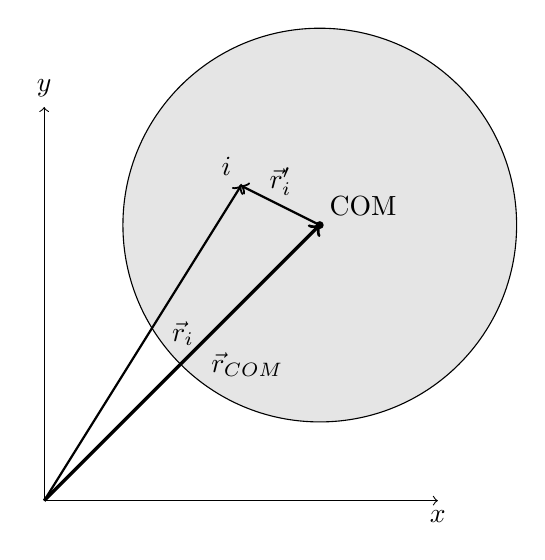
\begin{tikzpicture}[scale=5]
                \draw[<->] (0,1) |- (1,0);
                \node[above] at (0,1) {$y$};
                \node[below] at (1,0) {$x$};

                % TODO make this into a blob
                \filldraw[fill=black!10] (0.7,0.7) circle [radius=0.5];
                \fill (0.7,0.7) circle [radius=0.01];
                \draw[->,very thick] (0,0) -- (0.7,0.7);
                \node[above right] at (0.7,0.7) {COM};
                \node[below right] at (0.4,0.4) {$\vec{r}_\text{COM}$};

                \fill (0.5,0.8) circle [radius=0.005];
                \draw[->,thick] (0,0) -- (0.5,0.8);
                \node[above left] at (0.5,0.8) {$i$};
                \node[below right] at (0.3,0.48) {$\vec{r}_i$};
                \draw[->,thick] (0.7,0.7) -- (0.5,0.8);
                \node[above] at (0.6,0.75) {$\vec{r}_i^\prime$};
            \end{tikzpicture}
        \end{figure}
        We can label the position of particle $i$ inside the body as $\vec{r}_i$, and its position relative to the centre of mass at $\vec{r}_i^\prime$.
        Then
        \begin{equation}
            \vec{r}_i=\vec{r}_\text{COM}+\vec{r}_i^\prime.
        \end{equation}
        If we differentiate this equation, we can find the velocity of particle $i$:
        \begin{align}
            \vec{v}_i=\dot{\vec{r}}_i&=\dot{\vec{r}}_\text{COM}+\dot{\vec{r}}_i^\prime\\
            &=\vec{v}_\text{COM}+\vec{v}_i^\prime,
        \end{align}
        where $\vec{v}_i^\prime$ is the velocity of particle $i$ relative to the centre of mass.

        Let's look at the total kinetic energy of the system.
        It is the sum of the kinetic energy of all the constituent particles.
        \begin{align}
            K&=\frac{1}{2}\sum_{i=1}^N m_iv_i^2\\
            &=\frac{1}{2}\sum_{i=1}^N m_i(\vec{v}_\text{COM}+\vec{v}_i^\prime)^2\\
            &=\frac{1}{2}\sum_{i=1}^N m_i v_\text{COM}^2+\frac{1}{2}\sum_{i=1}^N m_i v_i^{\prime 2}+\frac{1}{2}\sum_{i=1}^N m_i(2\vec{v}_\text{COM}\cdot\vec{v}_i^\prime).
        \end{align}
        In the first term, $v_\text{COM}^2$ is constant and can be pulled out of sum, so the sum is simply the total mass $M$.
        The second term is the total kinetic energy in the centre of mass frame of reference, we call this the kinetic energy \textit{in} the centre of mass.
        Looking at the last term, we can once again take $\vec{v}_\text{COM}$ out of the sum, so the term becomes $\vec{v}_\text{COM}\cdot\sum_{i=1}^N m_i\vec{v}_i^\prime$.
        The sum is the total momentum in the centre of mass frame, which is zero.
        This can be justified by noting that in the centre of mass frame we have $\sum_{i=1}^N m_i\vec{r}_i^\prime=0$, so
        \begin{equation}
            \dv{}{t}\left(\sum_{i=1}^N m_i\vec{r}_i^\prime\right)=\sum_{i=1}^N m_i\vec{v}_i^\prime=0.
        \end{equation}
        Therefore the total expression for the kinetic energy of the system is
        \begin{equation}
            K=\frac{1}{2}M v_\text{COM}^2+\frac{1}{2}\sum_{i=1}^N m_i v_i^{\prime 2}.
        \end{equation}
        This is the kinetic energy associated with the total mass moving with speed $v_\text{COM}$ and the \textit{internal} kinetic energy from motion of particles relative to the centre of mass (the kinetic energy in the centre of mass).
        % TODO: prove that changes in kinetic energy are independent from choice of reference frame
        Depending on the problem, we can ignore the second term as it may not be relevant.
        For example, if we are examining the acceleration of a train, for the most part we don't care about the kinetic energy of objects within the vehicle.
        However, if we are looking at something that is rotating, like a flywheel for instance, we do care about the second term because there is a lot of motion relative to the centre of mass.

        Consider a system of two particles.
        \begin{figure}[H]
            \centering
            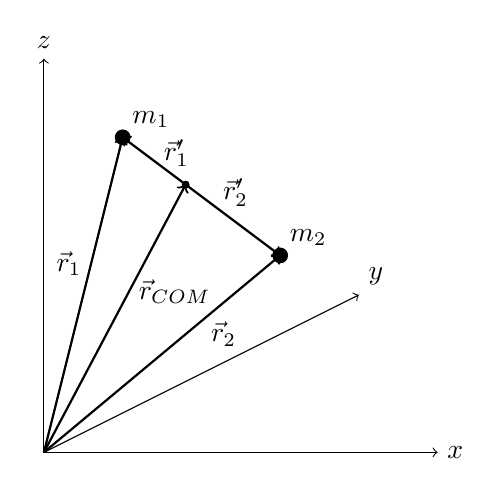
\begin{tikzpicture}[scale=5]
                \draw[<->] (0,1) |- (1,0);
                \draw[->] (0,0) -- (0.8,0.4);
                \node[right] at (1,0) {$x$};
                \node[above right] at (0.8,0.4) {$y$};
                \node[above] at (0,1) {$z$};

                \fill (0.2,0.8) circle [radius=0.02];
                \node[above right] at (0.2,0.8) {$m_1$};
                \fill (0.6,0.5) circle [radius=0.02];
                \node[above right] at (0.6,0.5) {$m_2$};
                \fill (0.36,0.68) circle [radius=0.01];
                \draw[->,thick] (0,0) -- (0.36,0.68);
                \node[right] at (0.216,0.408) {$\vec{r}_\text{COM}$};
                \draw[->,thick] (0,0) -- (0.2,0.8);
                \node[left] at (0.12,0.48) {$\vec{r}_1$};
                \draw[->,thick] (0,0) -- (0.6,0.5);
                \node[right] at (0.4,0.3) {$\vec{r}_2$};
                \draw[->,thick] (0.36,0.68) -- (0.2,0.8);
                \node[right] at (0.28,0.76) {$\vec{r}_1^\prime$};
                \draw[->,thick] (0.36,0.68) -- (0.6,0.5);     
                \node[right] at (0.43,0.66) {$\vec{r}_2^\prime$};
            \end{tikzpicture}
        \end{figure}
        In the centre of mass frame we have that $\sum_{i=1}^N m_1\vec{r}_i=0$, which in this case implies that
        \begin{equation}\label{eq:two-particle-momentum-relation}
            m_1\vec{r}_1=-m_2\vec{r}_2.
        \end{equation}
        We can define a vector $\vec{r}$ that points from $m_1$ to $m_2$, given by either
        \begin{gather}
            \vec{r}=\vec{r}_2-\vec{r}_1,\\
            \shortintertext{or equivalently,}
            \vec{r}=\vec{r}_2^\prime-\vec{r}_1^\prime.
        \end{gather}
        Substituting these relations into equation~\ref{eq:two-particle-momentum-relation} above and rearranging, we get
        \begin{equation}
            \vec{r}_1^\prime=\frac{-m_2}{m_1+m_2}\vec{r},\quad\vec{r}_2^\prime=\frac{m_1}{m_1+m_2}\vec{r}.
        \end{equation}

        Now let's look at the kinetic energy.
        In the centre of mass frame, it is
        \begin{equation}
            K^\prime=\frac{1}{2}m_1v_1^{\prime 2}+\frac{1}{2}m_2v_2^{\prime 2},
        \end{equation}
        were $\vec{v}_1^\prime=\dot{\vec{r}}_1^\prime$ and $\vec{v}_2^\prime=\dot{\vec{r}}_2^\prime$.
        Using the relations for $\vec{r}_1^\prime$ and $\vec{r}_2^\prime$ above, we get
        \begin{equation}
            \vec{v}_1^\prime=\frac{-m_2}{m_1+m_2}\vec{v},\quad\vec{v}_2^\prime=\frac{m_1}{m_1+m_2}\vec{v},
        \end{equation}
        where $\vec{v}=\dot{\vec{r}}$ is the \textbf{relative velocity} between the two particles.
        Therefore, the kinetic energy in the centre of mass frame becomes
        \begin{align}
            K^\prime&=\frac{1}{2}m_1\left(\frac{-m_2}{m_1+m_2}\vec{v}\right)^2+\frac{1}{2}m_2\left(\frac{m_1}{m_1+m_2}\vec{v}\right)^2\\
            &=\frac{1}{2}\frac{m_1m_2^2+m_1^2m_2}{(m_1+m_2)^2}v^2\\
            &=\frac{1}{2}\frac{m_1m_2(m_1+m_2)}{(m_1+m_2)^2}v^2\\
            &=\frac{1}{2}\mu v^2,
        \end{align}
        where we have defined the \textbf{reduced mass} $\mu$ as
        \begin{equation}
            \mu=\frac{m_1m_2}{m_1+m_2}.
        \end{equation}
        In a general inertial reference frame, the total energy (under the action of a conservative force) is given by
        \begin{equation}
            E=\frac{1}{2}Mv_\text{COM}^2+\frac{1}{2}\mu v^2+V(\vec{r}).
        \end{equation}

    \section{Non-conservative Forces}\label{sec:non-conservative-forces}
        Non-conservative forces are the opposite of conservative forces, that is they don't conserve energy.
        They can be characterised by failing to meet one or more of the conditions in definition~\ref{def:conservative-force}.
        I.e. for a non-conservative force, the work done depends on the path taken and there is no potential energy function.
        Another way of viewing this is that under the action of conservative forces, the work done along a path is equal to the negative of the work done by reversing along the path.
        So we get back the energy that we put in.
        But in the case of a non-conservative force like friction, we don't regain energy we put in by moving an object along a path.

        Let's look more closely at kinetic friction as an example.
        Consider a block sliding along a surface which is being slowed down by friction.
        \begin{figure}[H]
            \centering
            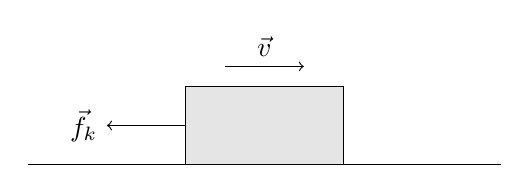
\begin{tikzpicture}
                \draw (0,0) -- (6,0);
                % TODO: add hatching effect to ground

                \filldraw[fill=black!10] (2,0) rectangle (4,1);
                \draw[->] (2,0.5) -- (1,0.5);
                \node[left] at (1,0.5) {$\vec{f}_k$};
                \draw[->] (2.5,1.25) -- (3.5,1.25);
                \node[above] at (3,1.25) {$\vec{v}$};
            \end{tikzpicture}
        \end{figure}
        The friction force $\vec{f}_k$ always points in the opposite direction to $\dd{\vec{r}}$, which points to the right.
        So, the work done by friction $W_f=\int_{\vec{r}_1}^{\vec{r}_2}\vec{f}_k\cdot\dd{\vec{r}}$ is \textit{always} negative.
        This is true for all paths, even closed ones, so we have
        \begin{equation}
            \oint\vec{f}_k\cdot\dd{\vec{r}}<0.
        \end{equation}

        Now let's add another conservative force and verify that energy is not conserved.
        Suppose the block is sliding down a slope, let $\vec{W}_x$ denote the component of weight acting parallel to $\dd{\vec{r}}$.
        \begin{figure}[H]
            \centering
            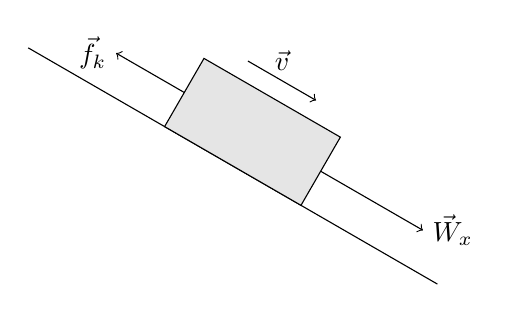
\begin{tikzpicture}
                \begin{scope}[rotate=-30]
                    \draw (0,0) -- (6,0);
                    % TODO: add hatching effect to ground

                    \filldraw[fill=black!10] (2,0) rectangle (4,1);
                    \draw[->] (2,0.5) -- (1,0.5);
                    \node[left] at (1,0.5) {$\vec{f}_k$};
                    \draw[->] (2.5,1.25) -- (3.5,1.25);
                    \node[above] at (3,1.25) {$\vec{v}$};
                    \draw[->] (4,0.5) -- (5.5,0.5);
                    \node[right] at (5.5,0.5) {$\vec{W}_x$};
                \end{scope}
            \end{tikzpicture}
        \end{figure}
        By the work-energy theorem, we can write
        \begin{align}
            \Delta K=\frac{1}{2}mv^2-\frac{1}{2}mv_0^2&=\int_{\vec{r}_0}^{\vec{r}}(\vec{f}_k+\vec{W}_x)\cdot\dd{\vec{r}}\\
            &=\int_{\vec{r_0}}^{\vec{r}}\vec{W}_x\cdot\dd{\vec{r}}+\int_{\vec{r_0}}^{\vec{r}}\vec{f}_k\cdot\dd{\vec{r}}\\
            &=-U(\vec{r})+\int_{\vec{r_0}}^{\vec{r}}\vec{f}_k\cdot\dd{\vec{r}}.
        \end{align}
        We know that the weight force is conservative, so we have replaced the integral with the potential energy function.
        Now let's rearrange this to get the final total energy on the left:
        \begin{equation}
            \frac{1}{2}mv^2+U(\vec{r})=\frac{1}{2}mv_0^2+\int_{\vec{r_0}}^{\vec{r}}\vec{f}_k\cdot\dd{\vec{r}}.
        \end{equation}
        Since the integral on the right is negative, the right hand side is always less than $\frac{1}{2}mv_0^2$, which is the initial energy.
        This implies
        \begin{equation}
            E_\text{final}<E_\text{initial},
        \end{equation}
        so energy is lost over time.

        In a general system, an object may be under the influence of multiple forces which can be conservative or non-conservative.
        If we split the resultant force on the system into a conservative part and a non-conservative part: $\vec{F}=\vec{F}_\text{conservative}+\vec{F}_\text{non-conservative}$, then using the work energy theorem again we can write
        \begin{align}
            \Delta K=W&=\int_{\vec{r}_1}^{\vec{r}_2}\vec{F}\cdot\dd{\vec{r}}\\
            &=\int_{\vec{r}_1}^{\vec{r}_2}\vec{F}_\text{conservative}\cdot\dd{\vec{r}}+\int_{\vec{r}_1}^{\vec{r}_2}\vec{F}_\text{non-conservative}\cdot\dd{\vec{r}}\\
            &=-\Delta U+W_\text{non-conservative}.
        \end{align}
        If we call the sum of kinetic energy and the potential energy from conservative forces $K+U$ the \textbf{mechanical energy} $E_\text{mech}$, then we get
        \begin{equation}
            \Delta E_\text{mech}=W_\text{non-conservative}.
        \end{equation}
        Consider the case where the non-conservative force is friction, so most of the work done is converted to heat, or \textbf{thermal energy}.
        So $W_\text{non-conservative}=-\Delta E_\text{thermal}$.
        This implies that we can write energy conservation as
        \begin{equation}
            \Delta E_\text{mech}+\Delta E_\text{thermal}=0.
        \end{equation}
        This implies that $\Delta E_\text{mech}\leq 0$, so the total mechanical energy in a closed system can only stay the same or decrease.
        % TODO: justify this
        We have basically just discovered the first and second laws of thermodynamics, but that is a topic for another time.
        If our system is not isolated and is acted on by an external force, we can say
        \begin{equation}
            \Delta E_\text{mech}+\Delta E_\text{thermal}=W_\text{ext},
        \end{equation}
        where $W_\text{ext}$ is the work done by the external force on the system.
        % TODO: give some examples of open systems
        \begin{example}
            A 2000kg elevator cable snaps at a height of 20m above a spring with $k=10,000$Nm$^{-1}$.
            Taking into consideration that the friction of the shaft walls exert a constant force of 15,000N to resist the fall of the elevator, what is the maximum compression of the spring?
            % TODO: write this example
        \end{example}

        % TODO: introduce power
        
        \begin{example}
            % TODO: provide justification for solution to this example
            Consider four possible paths of an object falling that start and end at the same height.
            Order the paths in terms of the final kinetic energy when there is no friction.
            What changes if there is friction?
            \begin{figure}[H]
                \centering
                \begin{tikzpicture}[scale=5]
                    \draw[<-] (0,1) node[left] {$h$} |- (2, 0);

                    \draw[shift={(0.2,0.9)}] (-0.06,-0.05) rectangle (0.06,0.05);
                    \draw[->,dashed] (0.2,0.8) -- (0.2,0.5);
                    \node[below] at (0.2,0) {A};
                    
                    \draw[shift={(0.56,0.9)},rotate=-68.2] (-0.06,-0.05) rectangle (0.06,0.05);
                    \draw (0.45,1) -- (0.85,0);
                    \node[below] at (0.65,0) {B};

                    \draw[shift={(1,0.9)},rotate=-73.3] (-0.06,-0.05) rectangle (0.06,0.05);
                    \draw (0.9,1) -- (1.2,0);
                    \node[below] at (1.05,0) {C};

                    \draw[shift={(1.33,0.9)},rotate=-83] (-0.06,-0.05) rectangle (0.06,0.05);
                    \draw (1.25,1) parabola bend (1.6,-0.2) (1.8,0);
                    \node[below] at (1.6,0) {D};
                \end{tikzpicture}
            \end{figure}
            With no friction, the final velocity is the same for all paths because the change in gravitional potential energy $U_g$ is the same.
            With friction, $v_A>v_B>v_C>v_D$.
        \end{example}

    \section{Collisions}\label{sec:collisions}
        A collision is an interaction between two objects over a short time interval.
        To solve these problems, we can use the concept of momentum conservation and energy conservation that we have been studying in the last two chapters.
        Consider two blocks sliding along a frictionles surface towards each other (1-dimensional problem).
        % TODO: include an explanation of how momentum is transferred from one block to another (through spring potential energy, etc.)
        The blocks have masses $m_1$, $m_2$ and velocities $v_1$, $v_2$ respectively.
        % TODO: include diagram to illustrate this
        What we want to find is the velocities of the blocks after the collision.
        To do this, we write the total momentum and kinetic energy before and after as
        \begin{align}
            \text{Before:}\quad&P=m_1v_1+m_2v_2\\
            & K=\frac{1}{2}m_1v_1^2+\frac{1}{2}m_2v_2^2\\
            \text{After:}\quad&P^\prime=m_1v_1^\prime+m_2v_2^\prime\\
            & K^\prime=\frac{1}{2}m_1v_1^{\prime 2}+\frac{1}{2}m_2v_2^{\prime 2}.
        \end{align}
        Total momentum is always conserved in collisions.
        On the other hand, depending on the forces involved during the collision, total kinetic energy may or may not be conserved.
        We call the case where it is conserved ``\textbf{elastic}'' and the case where it is not ``\textbf{inelastic}''. 

        In the case of elastic collisions, where total kinetic energy is conserved, we can write
        \begin{align}
            m_1v_1+m_2v_2&=m_1v_1^\prime+m_2v_2^\prime\\
            \frac{1}{2}m_1v_1^2+\frac{1}{2}m_2v_2^2&=\frac{1}{2}m_1v_1^{\prime 2}+\frac{1}{2}m_2v_2^{\prime 2}
        \end{align}
        This is a system of two equations for two unknowns, $v_1^\prime$ and $v_2^\prime$.
        We can solving this system using algebra, and the solution is
        \begin{align}
            v_1^\prime&=\frac{m_1-m_2}{m_1+m_2}v_1+\frac{2m_2}{m_1+m_2}v_2\\
            v_2^\prime&=\frac{2m_1}{m_1+m_2}v_1+\frac{m_2-m_1}{m_1+m_2}v_2.
        \end{align}
        Does this make sense?
        To examine whether this answer makes physical sense we can take some limits and see what happens to the solution.
        Set $v_2=0$ and then consider the limit where $m_1\gg m_2$.
        In this case, $v_1^\prime\to v_1$ and $v_2^\prime\to 2v_1$.
        % TODO: prove the limits properly
        This is like a bowling ball colliding with a ping-pong ball, the bowling ball keeps on going and the ping ball gets deflected in the same direction with twice the speed.
        % TODO: include diagrams for these
        If the two masses are equal, $v_1^\prime=0$ and $v_2^\prime=v_1$, which is like a perfect billiard ball collision.
        On the other hand, if $m_1\ll m_2$, $v_1^\prime\to -v_1$ and $v_2^\prime\to 0$.
        This corresponds to a ping-pong ball hitting a bowling ball at rest. It bounces off with the same speed in the opposite direction while the bowling ball stays still.

        If we transform the velocities into the centre of mass frame we get
        \begin{align}
            v_{1,\text{COM}}&=\frac{m_2(v_1-v_2)}{m_1+m_2}\\
            v_{2,\text{COM}}&=\frac{m_1(v_2-v_1)}{m_1+m_2}=-\frac{m_1}{m_2}v_{1,\text{COM}}\\
            v_{1,\text{COM}}^\prime&=-v_{1,\text{COM}}\\
            v_{2,\text{COM}}^\prime&=-v_{2,\text{COM}}.
        \end{align}
        % TODO: prove the bottom two formulae above
        So in the centre of mass frame, the two objects approach each other from opposite directions with velocities antiproportional to thei masses.
        After the collision, the magnitude of the velocities remains the same but they switch sign.

        In an inelastic collision, we only have conservation of momentum since some energy is lost to non-conservative forces in the collision.
        To solve the system, we need another constraint on the velocities after the collision.
        In the case where the \textit{maximum} kinetic energy is lost, which is when the objects stick together and move as a single body with velocity $v^\prime=v_1^\prime=v_2^\prime$.
        % TODO: prove that this is the case where maximum kinetic energy is lost
        This reduces the two equations for two unknowns that we had to solve before to one equation for one unknown.
        \begin{align}
            m_1v_1+m_2v_2&=m_1v^\prime+m_2v^\prime\\
            \implies v^\prime&=\frac{m_1v_1+m_2v_2}{m_1+m_2}.
        \end{align}
        Notice that $v^\prime$ is simply the centre of mass velocity.
        So, if we transform into the centre of mass frame the final velocity is 0
        \begin{equation}
            v_\text{COM}^\prime=v^\prime-v_\text{COM}=0.
        \end{equation}
        % TODO: need to distinguish between v_COM, the velocity in the COM frame, and v_COM, the COM velocity
        This means that in a \textbf{perfectly inelastic} collision seen from the centre of mass frame, the objects approach each other with the same velocities as in the elastic case, but then come together at rest at the origin.
        \begin{example}
            Golf ball on a basketball.
            % TODO: write this example
        \end{example}

\end{document}
